%%%%%%%%%%%%%%%%%%%%%%%%%%%%%%%%%%%%%%%%%
% Masters/Doctoral Thesis 
% LaTeX Template
% Version 1.43 (17/5/14)
%
% This template has been downloaded from:
% http://www.LaTeXTemplates.com
%
% Original authors:
% Steven Gunn 
% http://users.ecs.soton.ac.uk/srg/softwaretools/document/templates/
% and
% Sunil Patel
% http://www.sunilpatel.co.uk/thesis-template/
%
% License:
% CC BY-NC-SA 3.0 (http://creativecommons.org/licenses/by-nc-sa/3.0/)
%
% Note:
% Make sure to edit document variables in the Thesis.cls file
%
%%%%%%%%%%%%%%%%%%%%%%%%%%%%%%%%%%%%%%%%%

%----------------------------------------------------------------------------------------
%	PACKAGES AND OTHER DOCUMENT CONFIGURATIONS
%----------------------------------------------------------------------------------------

\documentclass[11pt, oneside]{Thesis} % The default font size and one-sided printing (no margin offsets)

\graphicspath{{Pictures/}} % Specifies the directory where pictures are stored

%-------------------------------------------------------
\usepackage{titlesec}
\titleformat{\chapter}{}{}{0em}{\bf\LARGE\thechapter.~}

\usepackage{etoolbox}
\makeatletter
\patchcmd{\chapter}{\if@openright\cleardoublepage\else\clearpage\fi}{}{}{}
\usepackage{float}

\usepackage{listings}
\usepackage{color}
\definecolor{mygreen}{rgb}{0,0.6,0}
\definecolor{mygray}{rgb}{0.5,0.5,0.5}
\definecolor{mymauve}{rgb}{0.58,0,0.82}
\lstset{ %
  backgroundcolor=\color{white},   % choose the background color
  basicstyle=\footnotesize,        % size of fonts used for the code
  breaklines=true,                 % automatic line breaking only at whitespace
  captionpos=b,                    % sets the caption-position to bottom
  commentstyle=\color{mygreen},    % comment style
  escapeinside={\%*}{*)},          % if you want to add LaTeX within your code
  keywordstyle=\color{blue},       % keyword style
  stringstyle=\color{mymauve},     % string literal style
}



%-------------------------------------------------------


\usepackage[square, numbers, comma, sort&compress]{natbib} % Use the natbib reference package - read up on this to edit the reference style; if you want text (e.g. Smith et al., 2012) for the in-text references (instead of numbers), remove 'numbers' 
\hypersetup{urlcolor=blue, colorlinks=false} % Colors hyperlinks in blue - change to black if annoying
\title{\ttitle} % Defines the thesis title - don't touch this

\begin{document}

\frontmatter % Use roman page numbering style (i, ii, iii, iv...) for the pre-content pages

\setstretch{1.1} % Line spacing of 1

% Define the page headers using the FancyHdr package and set up for one-sided printing
\fancyhead{} % Clears all page headers and footers
\rhead{\thepage} % Sets the right side header to show the page number
\lhead{} % Clears the left side page header

\pagestyle{fancy} % Finally, use the "fancy" page style to implement the FancyHdr headers

\newcommand{\HRule}{\rule{\linewidth}{0.5mm}} % New command to make the lines in the title page

% PDF meta-data
\hypersetup{pdftitle={\ttitle}}
\hypersetup{pdfsubject=\subjectname}
\hypersetup{pdfauthor=\authornames}
\hypersetup{pdfkeywords=\keywordnames}

%----------------------------------------------------------------------------------------
%	TITLE PAGE
%----------------------------------------------------------------------------------------

\begin{titlepage}
\begin{center}

\textsc{\LARGE \univname}\\[1.5cm] % University name
\textsc{\Large Text Mining Project}\\[0.5cm] % Thesis type

\HRule \\[0.4cm] % Horizontal line
{\huge \bfseries \ttitle}\\[0.4cm] % Thesis title
\HRule \\[1.5cm] % Horizontal line
 
\begin{minipage}{0.4\textwidth}
\begin{flushleft} \large
\emph{Author:}\\
\authornames % Author name - remove the \href bracket to remove the link
\end{flushleft}
\end{minipage}
\begin{minipage}{0.4\textwidth}
\begin{flushright} \large
\emph{Supervisor:} \\
\supname % Supervisor name - remove the \href bracket to remove the link  
\end{flushright}
\end{minipage}\\[3cm]
 
% \large \textit{A thesis submitted in fulfilment of the requirements\\ for the degree of \degreename}\\[0.3cm] % University requirement text
% \textit{in the}\\[0.4cm]
% \groupname\\\deptname\\[2cm] % Research group name and department name
 
{\large \today}\\[4cm] % Date
%\includegraphics{Logo} % University/department logo - uncomment to place it
 
\vfill
\end{center}

\end{titlepage}





%----------------------------------------------------------------------------------------
%	LIST OF CONTENTS/FIGURES/TABLES PAGES
%----------------------------------------------------------------------------------------

\pagestyle{fancy} % The page style headers have been "empty" all this time, now use the "fancy" headers as defined before to bring them back

\lhead{\emph{Table of Contents}} % Set the left side page header to "Contents"
\tableofcontents % Write out the Table of Contents

\lhead{\emph{List of Figures}} % Set the left side page header to "List of Figures"
\listoffigures % Write out the List of Figures

\lhead{\emph{List of Tables}} % Set the left side page header to "List of Tables"
\listoftables % Write out the List of Tables



%----------------------------------------------------------------------------------------
%	THESIS CONTENT - CHAPTERS
%----------------------------------------------------------------------------------------

\mainmatter % Begin numeric (1,2,3...) page numbering

\pagestyle{fancy} % Return the page headers back to the "fancy" style

% Include the chapters of the thesis as separate files from the Chapters folder
% Uncomment the lines as you write the chapters

% Chapter 1

\chapter{Introduction} % Main chapter title

\label{Chapter1} % For referencing the chapter elsewhere, use \ref{Chapter1} 

\lhead{ \emph{Introduction}} % This is for the header on each page - perhaps a shortened title

%----------------------------------------------------------------------------------------


%----------------------------------------------------------------------------------------






Text mining is used more and more to improve the way we get information or to enhance the way we perceive it. It is incorporated in many fields like politics, social media or improve existing technologies like spam filtering. Text classification is a branch of text mining. It is a classic task in natural language processing. Given a text document and a set of categories, the text classification algorithm must assign the text document into
one or more of the given text categories.\\
Nowadays social networks became a pillar for social interaction and Micro blogging is a new form of communication in which users can describe their current status in short posts distributed by instant messages, mobile phones, email or the Web. Twitter, a popular micro blogging tool has seen a lot of growth since it launched in October, 2006. It helps users to connect with their followers. The tweets from users are referred to as micro blogs because there is a 140 character limit imposed by Twitter for every tweet. This lets the users present any information with only a few words, optionally followed with a link to a more detailed source of information.
The project title in the domain of text classification, more precisely the task of
short text classification, which is more challenging than classic document classification. In
the proposed project title, we use the Twitter Political Corpus"\cite{website:data_set}. Given a tweet, the task
is to distinguish political tweets from non-political ones.

%----------------------------------------------------------------------------------------

% section 1

%----------------------------------------------------------------------------------------
\section{Motivations and goals}
A variety of techniques for supervised learning algorithms have demonstrated reasonable performance for text classification. The question is how would they perform for short text classification.
The project aims to fetch different classification settings, techniques and show how they perform in micro blog text classifications. 
Three different classifiers will be tested: Naïve Bayes, Maximum Entropy and Support Vector Machine.
%----------------------------------------------------------------------------------------

% section 2

%----------------------------------------------------------------------------------------
\section{Outline}
Figure \ref{fig:process_chain} shows the process undertaken in this project.
First we will see how the raw corpus is processed. Then how are the features extraction. Finally the classification results and discussions. 
\begin{figure}[H]
  \centering
  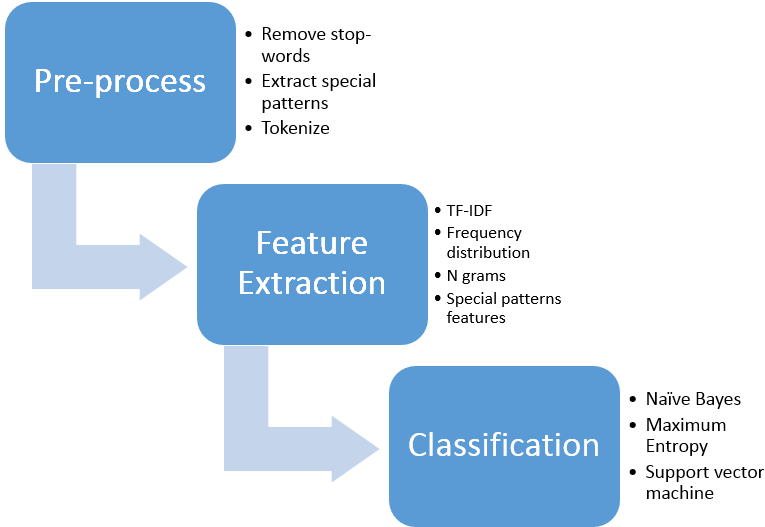
\includegraphics[width=150mm]{figures/process_chain.png}
  \caption{Process chain \label{fig:process_chain}}
\end{figure}
%% Chapter Template

\chapter{Motivations and Goals} % Main chapter title

\label{chapter2} % Change X to a consecutive number; for referencing this chapter elsewhere, use \ref{ChapterX}

\lhead{\emph{Motivations and Goals}} % Change X to a consecutive number; this is for the header on each page - perhaps a shortened title

%----------------------------------------------------------------------------------------
%	SECTION 1
%----------------------------------------------------------------------------------------




 
% Chapter Template

\chapter{Data set Processing} % Main chapter title

\label{Chapter3} % Change X to a consecutive number; for referencing this chapter elsewhere, use \ref{ChapterX}

\lhead{\emph{Data set Processing}} % Change X to a consecutive number; this is for the header on each page - perhaps a shortened title


Raw data is generally not well fitted for the needs of a project.  
This can be driven by the lack of attributes values or certain attributes of interest. 
Also real world data is noisy. It contains errors or outliers.  
Therefore the data needs to be processed. 
The next sections will show how the raw text is processed to get the most meaningful features out from it.
These features will be next used in the classification task. 
But first, a brief presentation of the data set is mandatory. 




\section{The data set}
The data set\cite{website:data_set} provides resources to develop learning algorithms that link political statements on Twitter to general opinions about government and politicians. It is composed of two files of tweets that have been hand labeled for their topics, specifically, discussing politics or not discussing politics.
Each file contains about 2000 tweets, one tweet per line. A line contains two fields separated by a single tab character: the label, and the text of the tweet:\\
\emph{POLIT     RT @AdamSmithInst Quote of the week: My political opinions lean more and more towards Anarchy }\\
\emph{NOT     @DeeptiLamba LOL, I like quotes. Feminist, anti-men quotes.}\\
The first file is a randomly selected set of 2000 tweets from Twitter's "spritzer" feed collected between June 1, 2009 and Dec 31, 2009. The second corpus is not selected from the entire feed, but rather randomly selected from a subset of tweets that contained at least one political keyword in each tweet.
The two labels are \emph{POLIT} (political) and \emph{NOT} (not political).\\
The two files are merged in the context of this work. In fact, on one side the \emph{Politics General Tweet Corpus} contains about 90\% of tweets labeled as \emph{non-political}. On the other side the \emph{Politics Keyword Tweet Corpus} contains about 90\% of tweets labeled as \emph{political}. If let so the classifier will have a good accuracy but in reality it won't do any classification task since 90\% of its entries are about one label.
By combining both corpora, the labels are equally distributed and a classifier can learn from it to predict political and non-political tweets. 
The two corpora are combined in the \textbf{\_tweets.txt} file.

%----------------------------------------------------------------------------------------
%	SECTION 1
%----------------------------------------------------------------------------------------

\section{Processing}


This section explains the assumptions and techniques used to process raw tweets.\\
For further testing and manipulations, the python code is available in the \textbf{preprocess.py} file.

%-----------------------------------
%	SUBSECTION 1
%-----------------------------------



\subsection{Special tweet patterns}
\label{sec:special_tweet_patterns}
Since in tweets there are many links, hashtags\footnote{Words that begin with \#}, users\footnote{Words that begin with @} and 'retweet' tokens, they need to be processed in a specific way.
At first, I made a hypothesis that links and 'retweet' tokens are relevant for political classification.
This assumption was made on these basis:
\begin{itemize}
\item Political tweets are important and thus they are highly 'retweeted'
\item Political tweets refer to important matters and tweets are limited in 140 characters. 
That's why they include links to explain the subject in more details. 
\end{itemize}
Unfortunately after seeing the distribution of these patterns in political and non-political tweets, it appears that they are equally scattered. As a result links and "retweet" tokens don't add any information Therefore they have been deleted in the process.

In second place, hashtags and users  are unique so meaningful for classification purpose.

%-----------------------------------
%	SUBSECTION 2
%-----------------------------------

  
\subsection{Delete stop words}
Not all words in a language are representative of a topic or a sentiment analysis. 
As a consequence they don't add information in the classification task.
These words are called stop words\cite{website:Stop_words}: 'They are words which are filtered out before or after processing of natural language data (text). There is no single universal list of stop words used by all processing of natural language tools, and indeed not all tools even use such a list'.   
Therefore a stop word list\footnote{stop\_words.py file} is created to fulfill the purpose of this work.\\
Generally English words are contracted. For example: \emph{'do not'} is written \emph{'don't'}. 
To prevent adding more entries to the stop word list, a contraction list\footnote{contractions.py file} that maps contracted words to their standard form has been created to expand these contractions.   
%-----------------------------------
%	SUBSECTION 3
%-----------------------------------
\subsection{Tokenize tweets }

The tokenization of tweets is processed using the \textit{nltk regexp tokenizer}\footnote{\href{http://www.nltk.org/_modules/nltk/tokenize/regexp.html}{URL: RegexpTokenizer }}.
This tool tokenizes text using a regular expression pattern.
The most important patterns that are implemented in the tokenizer are \verb/(\@\w*)+/ and \verb/(\#\w*)+/ as they prevent the tokenizer from deleting the \emph{\#} and \emph{@} symbols since they are important for the classification part.\\

After processing the data, tweets that have 1 or less token are deleted.




%-----------------------------------
%	SECTION 2
%-----------------------------------
\section{Feature extraction}
The final step for processing the data is feature extraction. 
This part is influenced by the machine learning algorithms that will be used to classify the tweets in the next step. 
In this way, feature engineering is really important and it strongly affects the final results. 
Also, this part is revisited as the project work progressed.\\
A bag of words feature set is used in this project. Further more part of speech tagging is not used because tweet text is not formal and too sparse. \\
For further testing and manipulations, the python code is available in the \textbf{feature\_extraction.py} file.


\subsection{Term Frequency - Inverse Document Frequency (tf-idf) features}
\label{sec:tfidf}
\emph{tf-idf}\cite{website:tfidf} is a numerical statistic that is intended to reflect how important a word is to a document in a collection or corpus. It is often used as a weighting factor in information retrieval and text mining. The tf-idf value increases proportionally to the number of times a word appears in the document, but is offset by the frequency of the word in the corpus, which helps to adjust for the fact that some words appear more frequently in general.\\
A \emph{scikit learn TfidfVectorizer}\footnote{\href{http://scikit-learn.org/stable/modules/generated/sklearn.feature_extraction.text.TfidfVectorizer.html}{URL: TfidfVectorizer }} is used to extract the \emph{tf-idf} feature set.

\subsection{Unigram frequency distribution features}
\label{sec:fd}
A bag of words feature set using frequency distribution counter is used from the \emph{nltk FreqDist}\footnote{\href{http://www.cs.bgu.ac.il/~nlpproj/hocr/doc/project.external.nltk_probability.FreqDist-class.html}{URL: FreqDist}} class.

\subsection{Tweets special patterns features}
\label{sec:special_patterns}
As mentioned in section (\ref{sec:special_tweet_patterns}) hashtags and users are unique and therefore they are relevant features for the classification task. 
However, not all the hashtags and users occur often in the data set. 
Moreover, not all tweets contain at least one hashtag or one user name.
In fact the data set contains 3259 tweets without hashtags and 2224 without user names. These designate respective rates of 84\% and 57\% of the tweets.
In this way only the most common hashtags and users are used as features. Also, these features are combined with a bag of words feature set to have a better impact on the classification process.\\  
The hashtag and users extractor can be tested on the \textbf{feature\_extraction.py} file.

\subsection{Bigram frequency distribution features}
\label{sec:bigram}
A bigram is a pair of consecutive written units such as letters, syllables, or words.
The bigrams are extracted using the \emph{nltk bigram}\footnote{\href{http://www.nltk.org/_modules/nltk/collocations.html}{URL: Collocations}} module.

% Chapter Template

\chapter{Classification Algorithms} % Main chapter title

\label{Chapter4} % Change X to a consecutive number; for referencing this chapter elsewhere, use \ref{ChapterX}

\lhead{\emph{Classification Algorithms}} % Change X to a consecutive number; this is for the header on each page - perhaps a shortened title

%----------------------------------------------------------------------------------------
%	SECTION 1
%----------------------------------------------------------------------------------------

Machine learning algorithms are the fundamental of all classification program. 
These algorithms are divided in two big families: the supervised learning and the unsupervised learning.
In this project only supervised learning models are used.
This section presents briefly the classification algorithms used in this work. 
\section{Naïve Bayes classifier}
A Naïve Bayes classifier\cite{website:Naive_Bayes_classifier} is a simple probabilistic classifier based on applying Bayes' theorem (from Bayesian
statistics) with strong (naive) independence assumptions. 
In simple terms, a naive Bayes classifier assumes that the presence (or absence) of a particular feature of a class is unrelated to the presence (or absence) of any other feature.
Depending on the precise nature of the probability model, naive Bayes classifiers can be trained very efficiently in a supervised learning setting.

\subsection{The Naïve Bayes probabilistic model}
Abstractly, the probability model for a classifier is a conditional model.
$$ P(C|F_1, \cdots, F_n) $$

Over a dependent class variable $C$ with a small number of outcomes or $classes$, conditional on several feature
variables $F_1$ through $F_n$ . The problem is that if the number of features $n$ is large or when a feature can take on a
large number of values, then basing such a model on probability tables is infeasible. Therefore the
model is formulated to make it more tractable using Bayes' theorem:
$$ P(C|F_1, \cdots, F_n) = \frac{p(C)p(F_1, \cdots, F_n|C)}{p(F_1, \cdots, F_n)}$$  The equation could be formulated as follow in a literal way $$posterior = \frac{prior * likelihood}{evidence}$$


%----------------------------------------------------------------------------------------
%	SECTION 2
%----------------------------------------------------------------------------------------

\section{Support Vector Machine}
A Support Vector Machine (SVM) is a discriminative classifier formally defined by a separating hyperplane. In other words, given labeled training data (supervised learning), the algorithm outputs an optimal hyperplane which categorizes new examples.
The figure \ref{fig:hyperplane} shows an example for a linearly separable set of 2D-points which belong to one of two classes.
\begin{figure}[H]
  \centering
  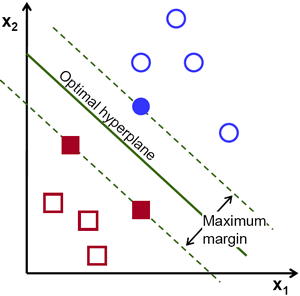
\includegraphics[width=60mm]{figures/optimal-hyperplane.png}
  \caption{Optimal hyperplane \label{fig:hyperplane}}
\end{figure}
The optimal hyperplane computedusing equation \ref{eq:hyperplane}:

\begin{equation}
\label{eq:hyperplane}
f(x) = \beta_{0} + \beta^{T} x
\end{equation}
Where $\beta$ is known as the weight vector and $\beta_{0}$ as the bias.

%----------------------------------------------------------------------------------------
%	SECTION 3
%----------------------------------------------------------------------------------------

\section{Maximum Entropy}
The maximum entropy classifier estimates probabilities
based on the principle of making as few
assumptions as possible, other than the constraints
imposed. Such constraints are derived from training
data, expressing some relationship between features
and outcome. The probability distribution
that satisfies the above property is the one with
the highest entropy. It is unique, agrees with the
maximum-likelihood distribution, and has the exponential
form :

\begin{equation}
\label{eq:maxent}
p(o|h) = \frac{1}{Z(h)}\prod_{j=1}^k\alpha_j^{f_j(h,o)}
\end{equation}

Where: 
\begin{itemize}
\item $o$ refers to the outcome
\item $h$ refers to the history or context.
\item $Z(h)$ is a normalization function.
\item $f_j(h,o)$ is a binary function.
\item $\alpha_j$ is estimated by a procedure called Generalized Iterative Scaling (GIS). This is an iterative method that improves the estimation of the parameters at each iteration.
\end{itemize} 
% Chapter Template

\chapter{Results and Discussion} % Main chapter title

\label{Chapter5} % Change X to a consecutive number; for referencing this chapter elsewhere, use \ref{ChapterX}

\lhead{\emph{Results and Discussion}} % Change X to a consecutive number; this is for the header on each page - perhaps a shortened title

%----------------------------------------------------------------------------------------
%	SECTION 1
%----------------------------------------------------------------------------------------

The evaluation task is the most crucial step for a project. This section explains how this process is conducted then discuss the results. But first, let's take a look at the standard machine learning evaluations methods. 

\section{Machine learning evaluation methods}
In pattern recognition and information retrieval with binary classification usually a confusion matrix is used to evaluate the systems performance.
A confusion matrix \textit{(Kohavi and Provost, 1998)} contains information about actual and predicted classifications done by a classification system. Performance of such systems is commonly evaluated using the data in the matrix.
\begin{theorem}
\label{confusion matrix}
\emph{Confusion Matrix}

$$\bordermatrix{~ & political & non-political \cr
                  political & Tp & Fn \cr
                  non-political & Fp & Tn \cr}$$
\end{theorem}
Where:
\begin{itemize}
\item $Tp$ (True positive): is the number of \textbf{correct} predictions that an instance is political.
\item $Fn$  (False negative): is the number of \textbf{incorrect} predictions that an instance is non-political.
\item $Fp$ (False positive): is the number of \textbf{incorrect} of predictions that an instance political.
\item $Tn$ (True negative): is the number of \textbf{correct} predictions that an instance is non-political.
\end{itemize}                  

From the Confusion Matrix \ref{confusion matrix}, different evaluation patterns are extracted:
\begin{equation}
\label{eq:accuracy}
Accuracy = \frac{Tp+Tn}{Tp+Tn+Fp+Fn}
\end{equation}
\begin{equation}
\label{eq:precision}
Precision = \frac{Tp}{Tp+Fp}
\end{equation}
\begin{equation}
\label{eq:recall}
Recall = \frac{Tp}{Tp+Fn}
\end{equation}
\begin{equation}
\label{eq:fmeasure}
F_1 = 2.\frac{precision . recall}{precision+recall} = \frac{2Tp}{2Tp+Fp+Fn}
\end{equation}


To balance the influence between precision and recall in
traditional text classification, we will adopt the $F_1$-Measure\ref{eq:fmeasure} as our precision's criterion to evaluate the performance of the classifiers in a
global aspect.


\section{Evaluation and Results}
First, the corpus is divided into a \emph{test set} and a \emph{training set} where the size of each one is respectively $ \frac{3}{4}.corpus$ and $ \frac{1}{4}.corpus$.

Then to model a real life situation the features are extracted only from the training set.




The evaluation aim is to answer the following questions: combine the following criterion to get the best classification settings:
\begin{itemize}
\item What is the optimal number of features for a classifier?\\
As the Maximum Entropy classifier needs a lot of time to learn, the maximum number of feature tested is capped at 200.
\item How does the different machine learning algorithms perform?
\item What is the best feature engineering pattern ?
\end{itemize}

The following sections will answer the above questions. In addition for further testing and manipulations, the python code is available in the \textbf{evaluation.py} file.


\subsection{Unigram feature}


Special patterns features\ref{sec:special_patterns} (hashtags and names) are extracted using the \emph{PatternsFeatures()} class in the \textbf{feature\_extraction.py} file. The 10 most frequent names and hashtags are taken. They are added to the bag of word feature set.
The results of the next subsections can be reproduced by running the \emph{unigram\_evaluation(lines)} function in the  \textbf{evaluation.py} file.\\
\subsubsection{Frequency distribution}
Figure \ref{fig:fd_eval} shows the results of the evaluation using the Frequency distribution\ref{sec:fd} feature selection. In fact, we can see that the $F_1$-Measure of the algorithms are relatively close for a certain number of features. Table \ref{tab:fd_results} summarizes the results.

\begin{table}[H]
\begin{tabular}{c|c|c}
~ & max f-measure & number of features \\
Naive Bayes		&			 0.891013 		&		190\\
Maximum entropy		&		 0.893058 		&		70\\
Support Vector Machine	&	 0.900000 		&		110\\
\end{tabular}
\caption{Best algorithms results using Frequency Distribution}\label{tab:fd_results}
\end{table}



\begin{figure}[H]
  \centering
  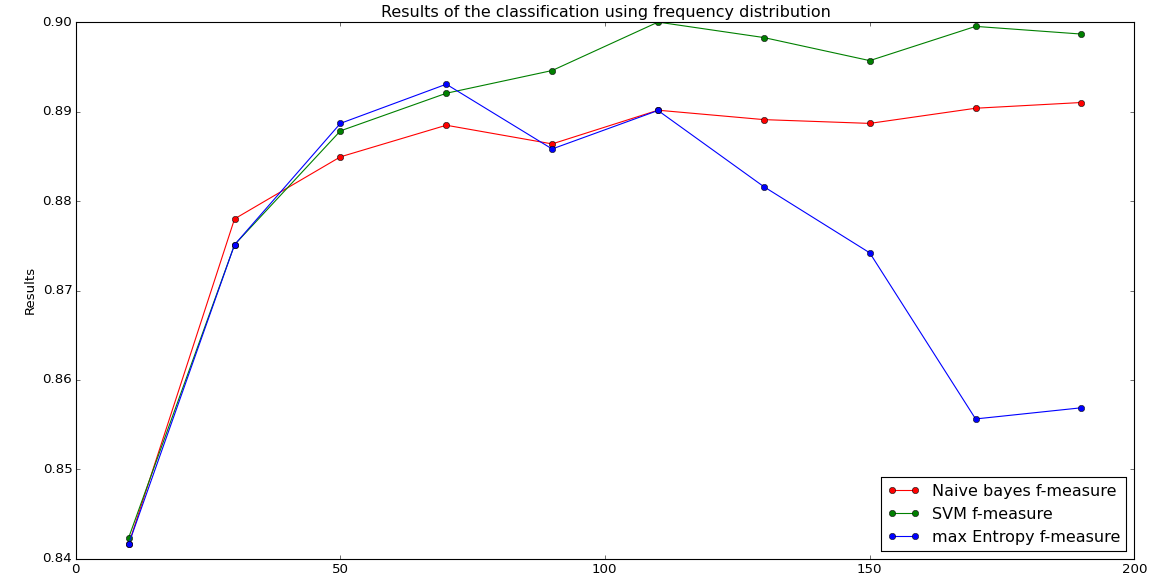
\includegraphics[width=160mm]{figures/result_fd_graph.png}
  \caption{Frequency Distribution Unigram F-Measure results for different number of features \label{fig:fd_eval}}
\end{figure}



\subsubsection{TF-IDF evaluation}
Figure \ref{fig:tfidf_eval} shows the results of the evaluation using the TF-IDF\ref{sec:tfidf} feature selection. In fact, we can see that the $F_1$-Measure of the algorithms are relatively close for a certain number of features. Table \ref{tab:tf-idf_results} summarizes the results.

\begin{table}[H]
\begin{tabular}{c|c|c}
		~	&				max f-measure 	& number of features \\
Naive Bayes			&		 0.894837 	&			190\\
Maximum entropy		&		 0.892791 	&			90\\
Support Vector Machine	&	 0.904215 	&			190\\
\end{tabular}
\caption{Best algorithms results using TF-IDF \label{tab:tf-idf_results}}
\end{table}

\begin{figure}[H]
  \centering
  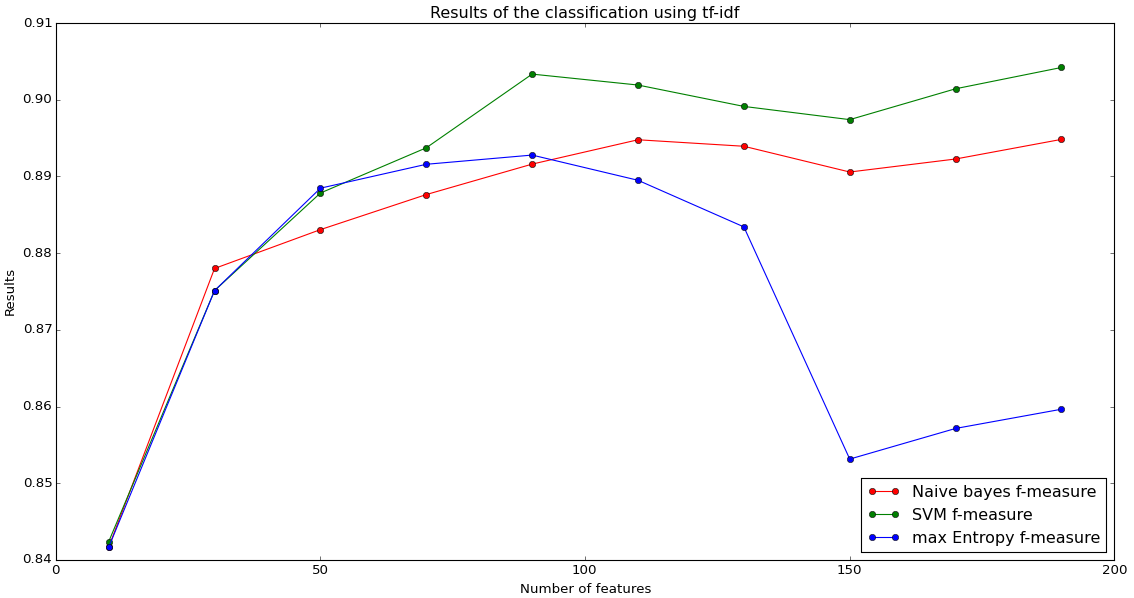
\includegraphics[width=160mm]{figures/result_tfidf_graph.png}
  \caption{tf-idf unigram F-Measure results for different number of features \label{fig:tfidf_eval}}
\end{figure}




\subsection{Bigram features}
\label{sec:bigram_results}
Figure \ref{fig:bigram_eval} shows that results of Bigram\ref{sec:bigram} features are constant. To have a better explanation of the result, the accuracy has been taken as well as the $F_1$-Measure. Table \ref{tab:tf-idf_results} summarizes the results.

\begin{table}[H]
\begin{tabular}{c|c|c}
		~	&				max f-measure 	& number of features \\
Naive Bayes			&		 0.754170 			&	170\\
Maximum entropy		&		 0.752347 			&	170\\
Support Vector Machine	&	 0.753623 			&	170\\
\end{tabular}
\caption{Best algorithms results using Frequency Distribution}\label{tab:bigram_results}
\end{table}


\begin{figure}[H]
  \centering
  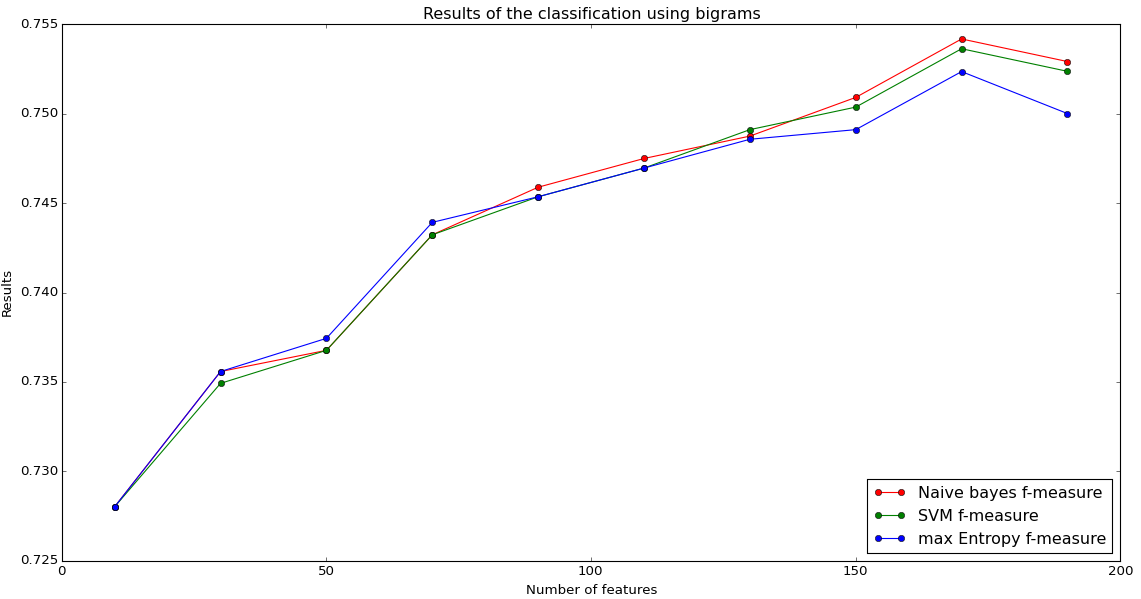
\includegraphics[width=160mm]{figures/bigram_results_graph.png}
  \caption{Bigrams F-Measure results for different number of features \label{fig:bigram_eval}}
\end{figure}

The results of this section can be reproduced by running the \emph{bigram\_evaluation(lines)} function in the  \textbf{evaluation.py} file.\\

\subsection{Combination of Unigrams and Bigrams }
\label{sec:combined_results}
The results shown in section \ref{sec:bigram_results} inform us that the overall outcome is independent from the number of bigrams used. At this end, only the 20 most frequent bigrams are used for this section.\\
Figure \ref{fig:uni_bi_eval} shows the results of the evaluation using Bigrams and Frequency Distribution feature selection. Table \ref{tab:tf-idf_results} summarizes the results.


\begin{table}[H]
\begin{tabular}{c|c|c}
		~	&				max f-measure 	& number of features \\
Naive Bayes				&	 0.818182 		&		190\\
Maximum entropy			&	 0.812893 		&		150\\
Suport Vector Machine	&	 0.824576 		&		200\\
\end{tabular}
\caption{Best algorithms results using Unigrams and Bigrams \label{tab:uni_bi_results}}
\end{table}

\begin{figure}[H]
  \centering
  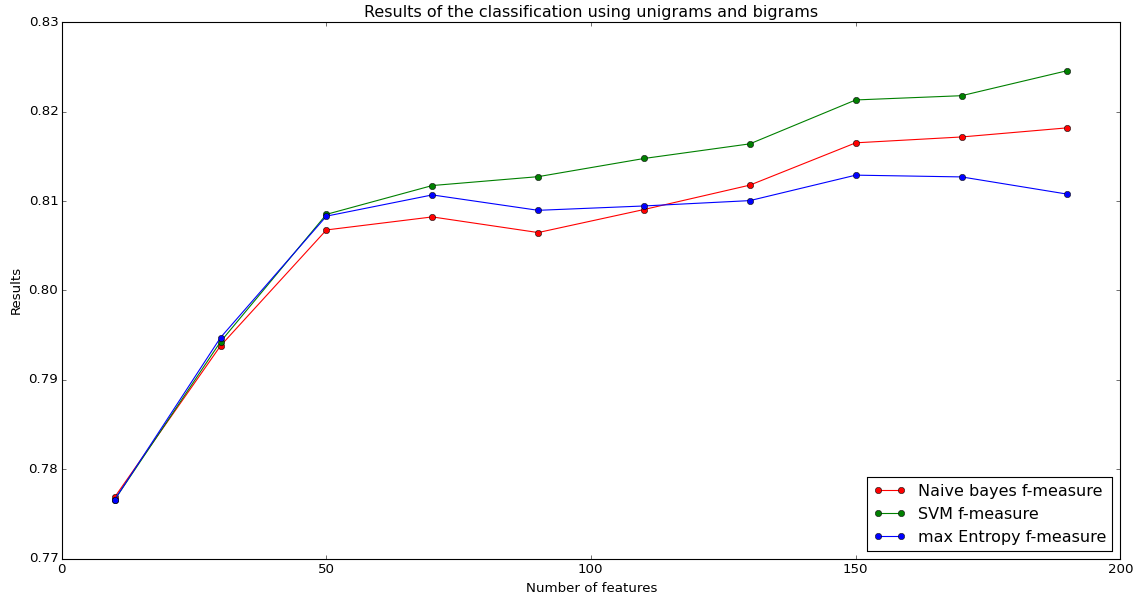
\includegraphics[width=160mm]{figures/combination_graph.png}
  \caption{Combination of Unigrams and Bigrams F-Measure results for different number of features \label{fig:uni_bi_eval}}
\end{figure}


The results of this section can be reproduced by running the \emph{uni\_and\_bi\_evaluation(lines)} function in the  \textbf{evaluation.py} file.\\

\section{Discussions}
\subsection{Result discussion}
The $F_1$-Measure results are relatively close in each test case. We can see that the Support Vector Machine classifier has a slight edge.\\
The unigram classification test the results show that the Support Vector Machine and Naïve Bayes classifiers reaches their best $F_1$-Measure for 190 features. This is an expected result because of the nature of these classifiers. However the maximum entropy falls down in $F_1$-Measure after reaching a peak at 70 features. This is explained by the motivation behind maximum entropy. In fact it says that one should prefer the most uniform models that satisfy any given constraint. By adding more features, the maximum entropy classifier needs more iterations to reach the best results. In this work the number of iterations for the Maximum Entropy classifier is 100 as it takes a lot of computation time.\\
The bigram classification test the results display an inferior result comparing to the unigram findings. This is explained by the frequency of a bigram. In fact the frequency  is very low compared to the unigrams.\\
This can be verified by running the next code.
\begin{lstlisting}[language=Python]
import preprocess
from nltk import FreqDist, bigrams
filename = "all_tweets.txt"
lines = preprocess.main(filename) 
all_tweets = " ".join([" ".join(line[1]) for line in lines])
print " 10 most frequent bigrams", FreqDist(bigrams(all_tweets.split(" "))).most_common(10)
print " 10 most frequent unigrams", FreqDist(all_tweets.split(" ")).most_common(10)
\end{lstlisting}
The outcome of the code of shown above reveal that the most frequent bigram appears 55 times although the most frequent unigram appears 429 times.
\begin{lstlisting}[language=Python]
10 most frequent bigrams  [((u'health', u'care'), 55), ((u'sarah', u'palin'), 37), ((u'president', u'obama'), 28), ((u'barack', u'obama'), 22), ((u'white', u'house'), 16), ((u'care', u'reform'), 16), ((u'bill', u'clinton'), 16), ((u'#tcot', u'#tlot'), 16), ((u'pres', u'obama'), 13), ((u'blog', u'post'), 13)]
 10 most frequent unigrams  [(u'obama', 433), (u'government', 260), (u'economy', 177), (u'afghanistan', 126), (u'2', 120), (u'good', 117), (u'senate', 115), (u'#tcot', 114), (u'congress', 110), (u'lol', 104)]
\end{lstlisting}

Finally, the combination of unigrams and bigrams has a fair result but not as good as unigram alone.
 
\subsection{Limitations}
The data set was collected between June 1, 2009 and Dec 31, 2009. The political subjects are dynamic and topics, key words change often. Therefor this model can't classify real time tweets.\\
Moreover this classification model works only on English tweets.\\
The special patterns features are limited since more than 50\% of the tweets does not contain a hashtag or/ and name.
\subsection{Improvements}
This project work can be improved, these are some ways:
\begin{itemize}
\item Test unsupervised learning algorithms.
\item Try to fetch new political tweets to keep the corpora up to date.
\end{itemize}
 
% Chapter Template

\chapter{Conclusion} % Main chapter title

\label{Chapter5} % Change X to a consecutive number; for referencing this chapter elsewhere, use \ref{ChapterX}

\lhead{\emph{Conclusion}} % Change X to a consecutive number; this is for the header on each page - perhaps a shortened title

%----------------------------------------------------------------------------------------
%	SECTION 1
%----------------------------------------------------------------------------------------

In this study we have analyzed a large social network in a
new form of social media known as micro blogging. 
The work showed results for some classic classification techniques applied to short text classification.
These results reveal that Support Vector Machine has the best $F_1$-Measure but the Maximum entropy needs less features than the Support Vector Machine to get almost the same outcome. Moreover, the unigrams features are better for this kind of classification.
\newpage 
%\input{Chapters/Chapter7} 

%----------------------------------------------------------------------------------------
%	THESIS CONTENT - APPENDICES
%----------------------------------------------------------------------------------------

%\addtocontents{toc}{\vspace{2em}} % Add a gap in the Contents, for aesthetics

%\appendix % Cue to tell LaTeX that the following 'chapters' are Appendices

% Include the appendices of the thesis as separate files from the Appendices folder
% Uncomment the lines as you write the Appendices
%\newpage
%% Appendix A

\chapter{Appendix Title Here} % Main appendix title

\label{AppendixA} % For referencing this appendix elsewhere, use \ref{AppendixA}

\lhead{Appendix A. \emph{Appendix Title Here}} % This is for the header on each page - perhaps a shortened title

Write your Appendix content here.
%\input{Appendices/AppendixB}
%\input{Appendices/AppendixC}

%\addtocontents{toc}{\vspace{2em}} % Add a gap in the Contents, for aesthetics

%\backmatter

%----------------------------------------------------------------------------------------
%	BIBLIOGRAPHY
%----------------------------------------------------------------------------------------
\nocite{*}
\label{Bibliography}

\lhead{\emph{Bibliography}} % Change the page header to say "Bibliography"

\bibliographystyle{unsrtnat} % Use the "unsrtnat" BibTeX style for formatting the Bibliography

\bibliography{Bibliography} % The references (bibliography) information are stored in the file named "Bibliography.bib"

\end{document}  